\newpage
\subsection{Mikrocontroller}
\label{subsec:Inbetriebnahme_Mikrocontroller}

Um das Anwenderprogramm auf dem Mikrocontroller (\textmu C) speichern zu können, ist es am angenehmsten, wenn dies direkt aus der Programmierumgebung geschehen kann. Als Programmierumgebung wird aufgrund des AVR-Chips die Software Atmel Studio 7.0 ausgewählt.

\subsubsection{Bootloader}

Ein Bootloader (BL) ermöglicht seitens \textmu C den Programmiervorgang über USB und stellt sicher, dass der frisch kompilierte Code in den Programmspeicher des \textmu C gelangt. Im Grunde ist der BL ein Code am Beginn des Programmablaufs, welcher entsprechend nach einem Reset aufgerufen wird. Innerhalb des BL-Codes wird für zwei Sekunden auf eingehende Daten der UART0-Schnittstelle gewartet.
%Wenn innerhalb von ca. zwei Sekunden keine Daten ankommen, wird das Anwenderprogramm gestartet. 
Wird innerhalb dieser zwei Sekunden ein Anwenderprogramm in Form eines HEX-Files an den Mikrocontroller gesendet, wird es gemäss stk500v2-Protokoll \todo{cite: http://ww1.microchip.com/downloads/en/Appnotes/doc2591.pdf} in den Flash-Speicher geladen.
%Nach dem Laden in den Flash-Speicher wird das neu geladene Programm gestartet. 
Aufgrund des BL geht es nach einem Reset des \textmu Cs zwei Sekunden, bis das eigentliche Programm startet.

Für den \textmu C des Cocktailmixers wird ein stk500v2-BL verwendet. Dieser kann über Github\footnote{https://github.com/arduino/Arduino-stk500v2-bootloader/blob/master/stk500boot.c
} heruntergeladen werden. Im File stk500v2.c befinden sich einige Anweisungen, welche Fuse- und Lock-Bits wann gesetzt werden müssen. Achtung, die Angaben haben im Falle des Cocktailmixers nur mit Abweichungen funktioniert (4096 words anstelle 1024). Durch Anpassen des start-Vektors auf den Programmspeicher und Setzen der korrekten Bootloader-Fuses wäre es möglich, den BL-Speicherplatz zu verkleinern um den Programmspeicher zu vergrössern.

%Wie der Flash-Speicher grob organisiert ist wird in Abbildung \ref{fig:Flash_Speicher_uC} gezeicht. Der Flash-Speicher für den Bootloader, wird in eine No-Read-While-Write Section geschrieben. Das Anwendungsprogramm in die Read-While-Write Section.

%\begin{figure}[h!]
%	\centering
%	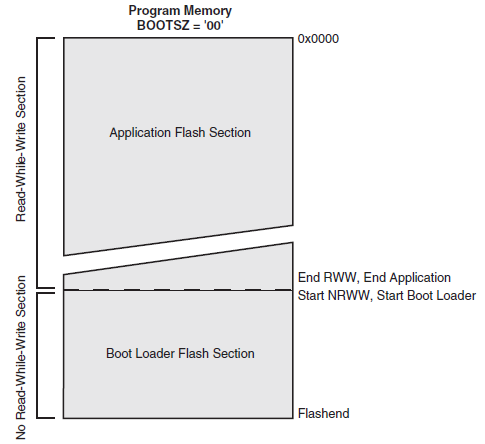
\includegraphics[width=0.8\textwidth]{graphics/Flash_Speicher_uC}
%	\caption{Flas-Speicher Mikrocontroller.}
%	\label{fig:Flash_Speicher_uC}
%\end{figure}
%\todo{cite: https://www.mikrocontroller.net/articles/AVR\_Bootloader\_in\_C\_-\_eine\_einfache\_Anleitung}
\subsubsection{Fuse-Bits}

%\begin{table}[h!]
%\center
%\begin{tabular}{|l|l|l|l|l|}
%\hline
%Bit & Register-Name & Default & Programmed & Mixer (0xFF)\\ \hline
%0 & BODLEVEL0 & 1 & 0 (1.8V) & 1\\
%1 & BODLEVEL1 & 1 & 0 (2.7V) & 1\\
%2 & BODLEVEL2 & 1 & 0 (4.3V) & 1\\
%3 & - & 1 & - & 1 \\
%4 & - & 1 & - & 1 \\
%5 & - & 1 & - & 1 \\
%6 & - & 1 & - & 1 \\
%7 & - & 1 & - & 1 \\ \hline
%\end{tabular}
%\label{tab:Extended_Fuses}
%\caption{Bits Etended Fuses.}
%\end{table}

%\begin{tabularx}{\textwidth}{ll|X}
%
%BODLEVEL0:2 				& : 	& Setzt die Brown-Out-Spannung. Sobald die Versorgungsspannung unterdiese Schwelle fällt, schaltet der uC aus. Für: 
%\begin{tabular}{lll}
%1.8V 		& = & 0b11111110\\
%2.7V 		& = & 0b11111101\\
%4.5V 		& = & 0b11111011\\
%disabled 	& = & 0b11111111
%\end{tabular}
%
%%\todo{cite: Atmel Datenblatt Seite 48}\\
%
%\end{tabularx}
%\todo{cite: Siehe Cites auskommentiert in Tabelle}

%\begin{table}[h!]
%\center
%\begin{tabular}{|l|l|l|l|l|l|l|l|l|}
%\hline
%Bit & Register-Name 	& Default 	& Programmed 							& Mixer (0xD0)\\ \hline
%0 	& BOOTRST  		& 1 			& 0 (Startet Bootloader bei Reset) 		& 0\\
%1 	& BOOTSZ0  		& 0 			& X (Definiert Bootloader-Speicherplatz) 	& 0\\
%2 	& BOOTSZ1  		& 0 			& X (Definiert Bootloader-Speicherplatz) 	& 0\\
%3 	& EESAVE  		& 1 			& 0 (Schützt EEPROM während Löschen) 	& 0\\
%4 	& WDTON 			& 1 			& 0 (Watchdog immer Ein)					& 1\\
%5 	& SPIEN 			& 0 			& 0 (Aktiviert ISP-Schnittstelle)		& 0\\
%6 	& JTAGEN 		& 0 			& 0 (Aktiviert JTAG-Schnittstelle) 		& 1\\
%7 	& OCDEN 			& 1 			& 0 (z.T Clock in Sleep-Modus) 			& 1\\ \hline
%\end{tabular}
%\label{tab:High_Byte_Fuses}
%\caption{Bits High-Byte-Fuses.}
%\end{table}

Da während dem Entwickeln die Möglichkeit bestehen soll, den Flash-Speicher per USB zu beschreiben, muss beim Aufstarten der BL aufgerufen werden. Dazu muss das BOOTRST-Bit aktiviert werden. Der Speicherplatz für den BL wird auf 4096 words gesetzt (anders als stk500v2 Erklärung). Das EEPROM soll beim Löschen des \textmu C geschützt bleiben, weshalb das EESAVE-Bit aktiviert wird. Da die ISP-Schnittstelle benötigt wird, um den BL zu schreiben und Fuse-Bits zu setzen, wird das SPIEN-Bit gesetzt.
%
%\begin{tabularx}{\textwidth}{ll|X}
%
%BOOTRST 	& : 	& 
%Nach Reset wird Programm von Bootloader-Memory-Section gestartet. Wenn ein Bootloader verwendet wird, um den Mikrocontroller zu flashen, muss dieses Bit aktiviert sein. \\ \hline
%
%%\todo{cite: https://embedds.com/all-you-need-to-know-about-avr-fuses/}\\
%
%BOOTSZ0:1 		& : &
%Definiert Bootloader-Grösse (je kleiner desto mehr Platz für Applikation). Grössen : 512, 1024,2048,4096 words.\\ \hline
%
%%\todo{cite: Atmel Datenblatt Seite 320}\\
%
%EESAVE 				& : & 
%Schütz EEPROM-Speicher währenddem der Chip gelöscht wird.\\ \hline
%
%%\todo{cite: https://embedds.com/all-you-need-to-know-about-avr-fuses/}\\
%
%
%WDON 				& : & 
%Forciert Chip-Reset, wenn nichts spezielles passiert.\\ \hline
%
%%\todo{cite: https://embedds.com/all-you-need-to-know-about-avr-fuses/}\\
%
%SPIEN 				& : & 
%Aktiviert die ISP-Schnittstelle. Don't touch!\\ \hline
%
%%\todo{cite: https://www.mikrocontroller.net/articles/AVR\_Fuses}\\
%
%JTAGEN 				& : & 
%Aktiviert die JTAG-Schnittstellt. Wird empfohlen auszuschalten wenn nicht benötigt.\\ \hline
%
%%\todo{cite: https://www.mikrocontroller.net/articles/AVR\_Fuses}\\
%
%OCDEN 				& : & 
%Ermöglicht gewissen Teilen des Clock-Systems während eines sleep-modus weiterhin zu laufen.\\
%
%%\todo{cite: Atmega2560 Datenblatt, Seite 327}\\
%
%\end{tabularx}
%\todo{cite: Siehe Cites auskommentiert in Tabelle}
%
%\begin{table}[h!]
%\center
%\begin{tabular}{|l|l|l|l|l|l|l|l|l|}
%\hline
%Bit & Register-Name 	& Default 	& Programmed 						& Mixer (0xF7)\\ \hline
%0 	& CKDIV8 		& 0 			& 0 (System-Clock-Prescaler = 8)		& 0\\
%1 	& CKOUT  		& 1 			& 0 (PE7 als System-Clock-Output) 	& 1\\
%2 	& SUT1			& 1 			& X (Aufstartzeit) 					& 0\\
%3 	& SUT0			& 0 			& X (Aufstartzeit) 					& 0\\
%4 	& CKSEL3			& 0 			& X (Frequenzbereich)				& 1\\
%5 	& CKSEL2			& 0 			& X (Frequenzbereich)				& 1\\
%6 	& CKSEL1			& 1 			& X (Frequenzbereich)				& 1\\
%7 	& CKSEL0			& 0 			& X (Aufstartzeit)					& 0\\
%\hline
%\end{tabular}
%\label{tab:Low_Byte_Fuses}
%\caption{Bits Low-Byte-Fuses.}
%\end{table}
%
Für den \textmu C verwenden wir einen 16MHz Full-Swing-Crystal-Oszillator, weshalb die Bits CKSEL3:1 auf 111 stehen müssen.
Die Aufstartzeit wird vorsorglich auf die längst mögliche Zeit eingestellt. Dies führt dazu, dass das Register CKSEL0 auf 0 und die Register SUT0:1 auf 00 gesetzt werden.
%
%
%\begin{tabularx}{\textwidth}{ll|X}
%
%CKDIV8 				& : 	& Setzt den Initialwert des System-Clock-Prescalers auf 8.
%\\ \hline
%
%%\todo{cite: Atmel Datenblatt Seite 48}\\
%
%CKOUT 				& : & Setzt den Pin PE7 als System-Clock-Output.
%\\ \hline
%
%%\todo{cite: Atmega Datenblatt Seite 327}\\
%
%SUT0:1 				& : & Setzt Parameter zur Aufstartzeit.
%\\ \hline
%
%%\todo{cite: Atmel Datenblatt Seite 42}\\
%
%CKSEL0:3 			& : & Setzt Parameter zum Oszillator (CKSEL1:3) und Aufstartzeit (CKSEL0).
%\\ \hline
%
%%\todo{cite: Atmel Datenblatt Seite 42}\\
%
%\end{tabularx}
%\todo{cite: Siehe Cites auskommentiert in Tabelle}
%
Der Brown-out-Detektor setzt den internen Reset, sobald die Versorgungsspannung unter einen Wert fällt. Wenn der Mikrocontroller ausfällt, während der TMC4671 noch aktiv ist, wird der Motor weiter gefahren. Dieses Risiko soll eingeschränkt werden, indem dieser Modus ausgeschaltet wird.

Die Lock-Bits müssen gesetzt werden, nachdem der BL in den Speicher geschrieben wurde. ''SPM ist nicht erlaubt, in den Anwenderbereich zu schreiben und LPM ist nicht erlaubt aus dem Applikationssktor zu lesen, wenn LPM aus dem Urlader-Bereich ausgeführt wird.''

\todo{cite : https://www-user.tu-chemnitz.de/~heha/viewchm.php/hs/ATmegaX8.chm/28.htm}
\newpage
Daraus folgt für die Fuse- und Lock-Bits die Einstellungen gemäss Tabelle \ref{tab:Fuse_und_Lock-Bits}. Siehe Anhang \ref{Appendix:Mikrocontroller} und \ref{Appendix:Atmel_Studio} für Details.

\begin{table}[h!]
\center
\begin{tabular}{|l|l|l|l|}
\hline
\textbf{Extended} & \textbf{High} & \textbf{Low} & \textbf{Lock}\\
\hline
0xFF & 0xD0 & 0xF7 & 0xCF\\
\hline
\end{tabular}
\caption{Tabelle Fuse- und Lock-Bits.}
\label{tab:Fuse_und_Lock-Bits}
\end{table}


\subsubsection{AVRdude in Atmel Studio einbinden}\label{subsubsec:avrdude_in_atmelstudio_einbinden}

AVRdude ist eine Software, mit der Atmel AVR Controller programmiert werden können. Sie schreibt den bereits kompilierten HEX-Code der Programmierumgebung über den Bootloader in den Flash-Speicher des Controllers. Hier gäbe es auch eine Methode, die Fuse- und Lock-Bits des \textmu C zu setzen.

\todo{https://www.mikrocontroller.net/articles/AVRDUDE}

Über einen Link\footnote{http://download.savannah.gnu.org/releases/avrdude/} kann eine Datei heruntergeladen werden in Form von \textcolor{blue}{avrdude-6.3-mingw32.zip}. Der gleichnahmige Ordner wird im Ordner \textcolor{blue}{C:\textbackslash Tools} gespeichert. Danach wird in AtmelStudio der Reiter ''\textcolor{blue}{Tools\textrightarrow External Tools}'' ausgewählt und ein neues Tool hinzugefügt. Im Falle des Atmega2560 geben wir die Commands gemäss Tabelle \ref{tab:AVRdude_commands} ein:

\begin{table}[h!]
\center
\begin{tabularx}{\textwidth}{|l|l|X|}
\hline
Title & : & Cocktailmixer \\
\hline
Command & : & C:\textbackslash Tools\textbackslash avrdude-6.1-mingw32\textbackslash avrdude.exe \\
\hline
Arguments: & : & -D -P \textcolor{red}{ COMx} -p ATMEGA2560 -c wiring -b 115200 -U flash:w:\$(TargetDir)\$(TargetName).hex:i\\
\hline
\end{tabularx}
\caption{AVRdude Commands}
\label{tab:AVRdude_commands}
\end{table}

Der entsprechende \textcolor{red}{ COMx}-Port des zu flashenden Gerätes (Atmega2560) muss mit dem Geräte-Manager ermittelt werden.

\todo{cite Herr Meier Skript mc1}


Sämtliche Tabellen aus dem Datenblatt und Screenshots aus Programmierumgebung, welche mit dem Setzen der Fuse- und Lock-Bits oder Programmierung des \textmu C zusammenhängen, sind im Anhang Kapitel \ref{Appendix:Mikrocontroller} angefügt.

\subsubsection{Vorgehen}\label{subsubsec:Inbetriebnahme_uC_Vorgehen}

\begin{enumerate}
\item Als Erstes wurden die Fuse-Bits gesetzt. Dies geschah über den Reiter:\newline
\textcolor{blue}{AtmelStudio \textrightarrow Tools \textrightarrow Device programming \textrightarrow Fuses} (siehe Abbildung \ref{fig:AtmelStudio_Fuses}) \newline
Es wurde darauf geachtet, dass der AVR mkII ausgewählt wurde und der Gerätecode des Atmega2560 ausgelesen werden konnte.
\newline
\item Als Zweites wurde der Bootloader installiert. Dies geschah unter:\newline
\textcolor{blue}{AtmelStudio \textrightarrow Tools \textrightarrow Device programming \textrightarrow Memory} (siehe Abbildung \ref{fig:AtmelStudio_Program_Bootloader}) \newline
Hier wird ein stk500v2-BL verwendet, kann aber auch abweichen. (Entsprechende Anpassungen nötig, nicht Teil dieses Projektes.)\newline
\item Als Drittes wurden die Lock-Bits gesetzt unter:\newline
\textcolor{blue}{AtmelStudio \textrightarrow Tools \textrightarrow Device programming \textrightarrow Lock-Bits} (siehe Abbildung \ref{fig:AtmelStudio_Locks})\newline
Diese sollten nicht mehr geändert werden. Bei jedem Brennen des BL wieder zu setzen.\newline
\item Ggf. USB-Firmware installieren auf dem USB-UART-Converter. (Nicht Teil dieses Projektes.)\newline
\item Mikrocontroller mit der kompillierten Software (Cocktailmixer.HEX) programmieren.\newline
\textcolor{blue}{AtmelStudio \textrightarrow Tools \textrightarrow Cocktailmixer})\newline
Alternativ direkt mit ISP-Programmer wie in Schritt 2 (ohne Bootloader, Programmcode an start-Vektor des \textmu Cs.):\newline
\textcolor{magenta}{z.B C:\textbackslash Users\textbackslash DaU\textbackslash Software\textbackslash Cocktailmixer\textbackslash Cocktailmixer\textbackslash Debug\textbackslash Cocktailmixer.HEX}
\end{enumerate}

Das Setzen der Fuse- und Lock-Bits sowie das brennen des Bootloaders kann mit einem AVR MKII Programmer in Atmel Studio gemacht werden. Alternativ gibt es einen Weg, den USB-Treiber (Atmega16U2) eines Arduino Uno mit einer entsprechenden Firmware zu laden, sodass dieser als Programmer verwendet werden kann\footnote{https://www.instructables.com/id/Turn-Arduinos-Serial-Converter-Into-AVRISP-MkII-Cl/}.

Für die Inbetriebnahme des Mikrocontrollers wurde der Alternativweg gewählt. Die Ergebnisse können sich zeigen lassen. Der Mikrocontroller ist programmierbar und erste Tests mit der Software waren erfolgreich, das Programm wurde auch ordnungsgemäss gestartet. Dies wurde geprüft, indem der während dem Projekt 5 erarbeitete Code hochgeladen wurde.

Wird der Mikrocontroller per Reset-Button neu gestartet, dauert es aufgrund des Bootloaders 2s, bis der Programmcode gestartet wird. Während dieser Zeit wartet der Bootloader auf einkommende Daten, welche auf den Flash-Speicher geschrieben werden sollen. Danach startet das Programm, sollten keine Daten kommen.

\subsubsection{Messungen}

Die Messung des Oszillator-Eingangs ergab eine saubere harmonische Schwingung mit 16MHz, abgebildet in Abbildung \ref{fig:Crystal_Swing}. 

\begin{figure}[h!]
\center
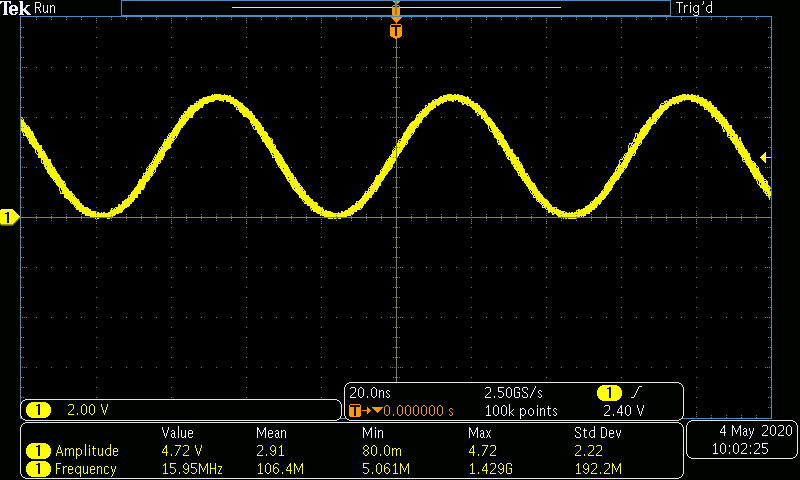
\includegraphics[width = 0.8\textwidth]{graphics/Crystal_Swing}
\caption{Schwingung des Oszillators}
\label{fig:Crystal_Swing}
\end{figure}